\documentclass[a4paper, 12pt]{report}
\usepackage[utf8]{inputenc}
\usepackage[T1]{fontenc}

\usepackage{xcolor}
\usepackage{afterpage}

\usepackage{relsize}
\usepackage{moresize}

\usepackage{graphicx}
\usepackage{geometry}

% [CHANGE] The title of your thesis. If your thesis has a subtitle, then this
% should appear right below the main title, in a smaller font.
\newcommand{\theTitle}{Quadratic Forms in \\
\vspace{0.5em}
Convolutional Neural Networks}
\newcommand{\theSubTitle}{}


% [CHANGE] Your full name. In case of multiple names, you can include their
% initials as well, e.g. "Robin G.J. van Achteren".
\newcommand{\theAuthor}{Peter Adema}

% [CHANGE] Your student ID, as this has been assigned to you by the UvA
% administration.
\newcommand{\theStudentID}{14460165}

% [CHANGE] The name of your supervisor(s). Include the titles of your supervisor(s),
% as well as the initials for *all* of his/her first names.
\newcommand{\theSupervisor}{Dr. ir. R. van den Boomgaard} % Dr. Ing. L. Dorst

% [CHANGE] The address of the institute at which your supervisor is working.
% Be sure to include (1) institute (is appropriate), (2) faculty (if
% appropriate), (3) organisation name, (4) organisation address (2 lines).
\newcommand{\theInstitute}{
Informatics Institute \\ %Institute for Logic, Language and Computation
Faculty of Science\\
University of Amsterdam\\
Science Park 900 \\ 
1098 XH Amsterdam 
}

% [CHANGE] The semester in which you started your thesis.
\newcommand{\theDate}{Semester 2, 2024-2025}



\usepackage[shortlabels]{enumitem}
\usepackage{graphicx}
\usepackage{hyperref}
\usepackage{amsmath}
\usepackage{amssymb}
%\usepackage{apacite}
\usepackage{caption}
\usepackage{listings}
\usepackage{xcolor}
\def\comment#1{\color{red}#1\color{black}}
\usepackage{bbold}

\begin{document}
\pagestyle{empty}
\begin{center}

\vspace{2.5cm}


\begin{Huge}
% see definition at beginning of document
\theTitle
\end{Huge} \\

\vspace{0.5 cm}

\begin{Large}
\theSubTitle
\end{Large}

\vspace{1.5cm}

% see definition at beginning of document
\theAuthor\\
% see definition at beginning of document
\theStudentID

\vspace{1.5cm}

% [DO NOT CHANGE]
Bachelor thesis\\
Credits: 18 EC

\vspace{0.5cm}

% [DO NOT CHANGE] The name of the educational programme.
Bachelor \textit{Kunstmatige Intelligentie} \\
\vspace{0.25cm}

\includegraphics[width=0.075\paperwidth]{figures/uva_logo} \\
\vspace{0.1cm}

% [DO NOT CHANGE] The address of the educational programme.
University of Amsterdam\\
Faculty of Science\\
Science Park 900\\
1098 XH Amsterdam

\vspace{2cm}

\emph{Supervisor}\\

% see definition at beginning of document
\theSupervisor

\vspace{0.25cm}

% see definition at beginning of document
\theInstitute

\vspace{1.0cm}

% see definition at beginning of document
\theDate

\end{center}
\newpage



\pagenumbering{arabic}
\setcounter{page}{1}
\pagestyle{plain} 

\newgeometry{a4paper, textwidth=400.0pt, textheight=740.0pt}
\chapter{Introduction}
\comment{\ldots\ldots}

\chapter{Background}
First, some mathematical formalisms must be covered to understand the concepts discussed in the implementation and results sections, namely fields and semifields, construction of positive definite matrices and efficient calculation of quadratic forms.

\section{Convolutional stencil}
At the core of a convolutional neural network is the convolutional operation $f*g$, where, save for a handful of separable functions, $g$ is approximated with a fixed-size discrete kernel. This kernel may be fixed, but most modern machine learning architectures learn the kernel as part of the model's parameters (see \cite{introconvnets} for an introduction). As such, the calculation for the output of a single (discrete) pixel is of the form:
\begin{align*}
(f*g)[x] = \sum_{y\in\mathcal{I}} f[x-y]\; g[y]	, \textrm{ where } \mathcal{I} \textrm{ is the set of indices valid for }g,
\end{align*}
\comment{I explicitly wanted to discuss the discrete case here, as I wanted to link it to the discrete weighed average. I could also work for the continuous (integral) case for both sections, but considering I never use PDEs or other continuous constructs, do you think it has added value? (might make it harder to follow, but if it's useful\ldots) \\}
possibly also summing over multiple input channels. An access pattern such as this, where the new value of a pixel depends on a fixed window of its neighbours, is referred to as a stencil computation \cite{fortranstencils}, and as such, the stencil computation performed by the discrete convolution operator will hereafter be referred to as the convolutional stencil, while the discrete version of $g$ will be referred to as the (convolutional) kernel.

\section{Fields, semifields and weighted reductions}
In the convolutional stencil, a part of the image is multiplied element-wise with a kernel, and the resulting values are summed to obtain an activation for that point. However, while we typically use scalar addition and multiplication in this calculation, it is also possible to use different operators in the reduction by defining a different field in which the reduction is done. In this section, we will briefly look at the concept of fields insofar as they are relevant to the reduction in the convolutional stencil.

In mathematics, a field is a set of values with a pair of operators that work on those values: one operator corresponds to the concept of addition, and one operator corresponds to the concept of multiplication. Fields are, in effect, a generalisation of standard addition and multiplication on integers or reals and allow for describing a set of values other than typical scalars or an alternate method for combining typical numbers. Formally, a field can be described as a tuple $(\mathcal{F}, \oplus, \otimes)$, where the operators $\oplus$ and $\otimes$ are of the type $\mathcal{F}\times\mathcal{F}\rightarrow\mathcal{F}$. Furthermore, the operators $\oplus$ and $\otimes$ are both beholden to the field axioms: informally, a set of rules to ensure they act 'similarly' to standard scalar addition and multiplication. These field axioms are as follows (\cite{beachy2006abstract}, page 120):
\begin{align}
\textrm{Associativity for $\oplus$ and $\otimes$: }&\forall a,b,c\in \mathcal{F}~~  a \circ (b \circ c) = (a\circ b) \circ c \\ 
\textrm{Commutativity for $\oplus$ and $\otimes$: }&\forall a,b\in \mathcal{F}~~~~~ a\circ b = a  \circ a \\
\oplus\textrm{ identity: }& \exists \mathbb{0}~\forall a\in \mathcal{F}~~~ a\oplus \mathbb{0} = a \\ 
\otimes\textrm{ identity: }& \exists \mathbb{1}~\forall a\in \mathcal{F}~~~ a\otimes \mathbb{1} = a \\ 
\oplus\textrm{ has inverse elements: }& \forall a~\exists b\in \mathcal{F}~~~ a\oplus b = \mathbb{0}  \\ 
\otimes\textrm{ has inverse elements: }& \forall a~\exists b\in \mathcal{F}~~~ a\otimes b = \mathbb{1}  \\ 
\textrm{Distributivity: }&\forall a,b,c\in \mathcal{F}~~ a\otimes (b \oplus c) = (a\otimes b)\oplus(a\otimes c)
\end{align}

One use case for fields in machine learning is to describe a weighted reduction (as in a kernel-based convolution) more generally. To better understand this, suppose we have a sequence of numbers $\mathbf{a} \in \mathcal{F}^N$  (e.g. $[10, 12, 17]$), which we wish to summarise into a single value. This $\mathbf{a}$ could then represent the (flattened) neighbourhood around $x$ that is extracted during the calculation of the correlational stencil $(f \star g)(x)$. We could accomplish the summarisation by repeatedly applying an operator $\oplus$ (e.g. $10 \oplus 12 \oplus 17$): this would then be referred to as a reduction with $\oplus$ and could also be written as $\bigoplus_{i\in \mathcal{I}}\mathbf{a}[i]$. Typically, we also require that $\oplus$ be associative and commutative (an abelian group, see \cite{beachy2006abstract}), enabling the parallelisation of the reduction by reassociating the $\oplus$ and performing some operations out of order \cite{ppad}. However, we may also wish to weigh some terms of the sequence more heavily in the summary: for this purpose, we could use a second operator $\otimes$ with a second sequence of weights $\mathbf{w} \in \mathcal{F}^N$ (as with the kernel in a convolution or correlation) and write $\bigoplus_{i\in \mathcal{I}}\mathbf{a}[i] \otimes \mathbf{w}[i]$. 

We can see that a weighted reduction can be implemented on a field $(\mathcal{F}, \oplus, \otimes)$, as the requirements for a weighted reduction are few and a subset of the field axioms. Therefore, defining a field with appropriate operators is a sufficient condition for performing a weighed reduction. However, it is not a necessary condition: as defined above, the field axioms are overly strict compared to what is necessary for the weighted reduction, and we could relax some assumptions to obtain, e.g., a semiring. In practice, though, the operators typically used for reduction fulfil most, if not all, of the requirements for a field. As such, the spaces in which reductions are performed are typically described as a semifield: a field that does not neccesarily have an additive inverse, relaxing assumption 5 from the previous definition \cite{bellaardaxiomatic}.

Finally, since weighted reduction can be performed in any semifield, we can perform an operation similar to the convolutional stencil in any semifield. If we see $\mathbf{a}$ as an image neighbourhood around $x$ from $f$, and $\mathbf{w}$ as a kernel $g$, then we can see
\begin{align*}
\mathbf{a}[i] &= f(x + i) \textrm{ and } \mathbf{w}[i] = g(i) \textrm{, so} \\
\bigoplus_{i\in \mathcal{I}}\mathbf{a}[i] \otimes \mathbf{w}[i]
&= \bigoplus_{y\in \mathcal{I}}f[x+y] \otimes g[y] \\
\end{align*}
This looks very similar to a correlation, and we can therefore chose to define the (discrete) semifield correlation operator $\textcircled{$\star$}$ to mean exactly this:
\begin{align*}
	(f \star g)[x] &= \sum_{y\in\mathcal{I}}f[x+y]\; g[y]\\
	(f ~\textcircled{$\star$}~ g)[x] &=\bigoplus_{y\in \mathcal{I}}f[x+y] \otimes g[y] \textrm{ in some semifield $(\mathcal{F}, \oplus, \otimes)$}
\end{align*}
\section{Nonlinear semifields from computational morphology}
Knowing that convolutional stencils are weighted reductions and that weighted reductions can be implemented in all semifields, we can examine if there are other semifields in which we can perform a convolution or correlation than the standard linear field. For this, we can take inspiration from computational morphology, the mathematics of object and function shapes.

Two core operations from computational morphology are dilation and erosion, where dilation corresponds with 'making a function larger' (scaling the umbra of a function), and erosion is 'making a function smaller'. The result of dilation is shown in Fig. \ref{fig:dil-illust}. Examining the local effects of dilation more closely, we can see that it is somewhat similar to taking a local maximum. This similarity can be made more concrete by understanding the formula for discrete dilation: 
$$f \boxplus g \textrm{, where }(f \boxplus g)[x] = \max_{y\in\mathcal{I}} \left(f(x+y) + g(y)\right)$$

\comment{Is there a need to use the supremum in the discrete case?}

Here, $f$ is the function (or object or image) to be dilated, and $g$ is a concave structuring function describing how the dilation will occur. An intuitive explanation would be to see the structuring function $g$ as a (negated) distance function and dilation $\boxplus$ as the operation that takes the highest value also 'close' to $x$. If $g$ is a step function with a value zero near its centre and $-\infty$ outside (Fig. \ref{fig:dil-illust}, first row), we can see that this is precisely taking the maximum value within the range specified by $g$. However, we may also wish to use a quadratic (Fig. \ref{fig:dil-illust}, second row) or other concave function as $g$. Depending on $f$, we may still be able to perform the dilation with an arbitrary $g$ (using algebraic solutions, or leveraging separability), but to compute the dilation in the general case we may wish to clip all functions $g$ to be above $-\infty$ in only a constrained domain (Fig. \ref{fig:dil-illust}, third row). The dilation with the clipped version of $f\boxplus g_{clipped}$ could then be seen as an approximation of the dilation $f\boxplus g$ with the full (unclipped) $g$, while having the advantage that the set of relevant indices $\mathcal{I}$ is bounded in size.

\begin{figure}[h!]
  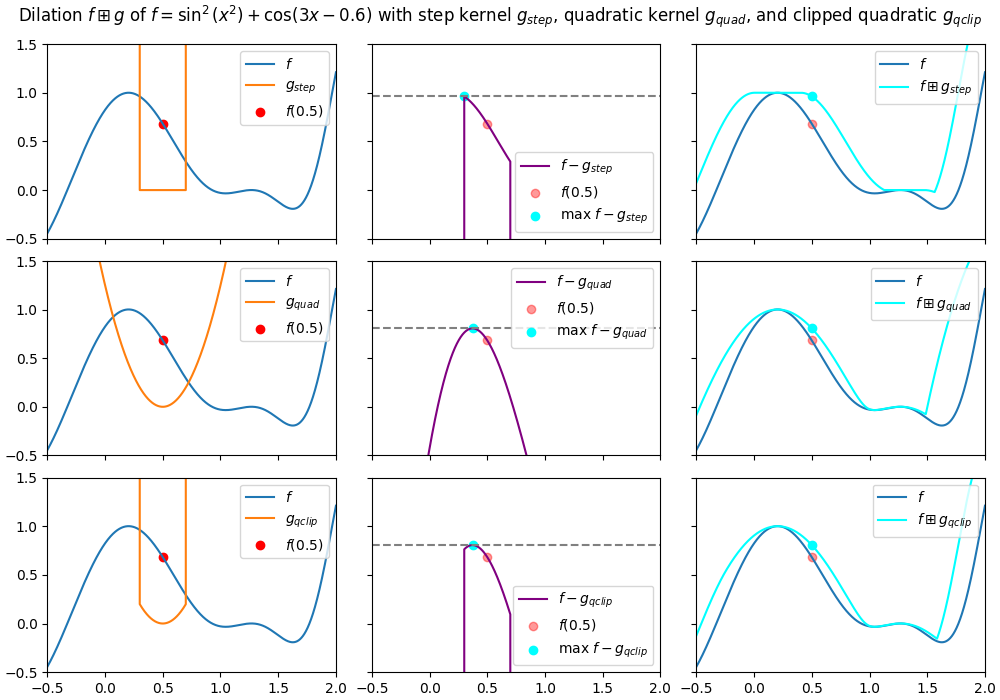
\includegraphics[width=\textwidth]{figures/dilation_illustration.png}
  \caption{Illustration of the effects of dilation with three kernels on a sinusoidal $f$. $g_{step}=0$ in a region of size 0.5, $-\infty$ outside. $g_{quad}=-5x^2$, and $g_{qclip}=g_{quad}+g_{step}$. \\An alternative intuition for dilation is also illustrated, corresponding with 'lowering' a negated version of $g'$ down towards the point $x$ until it intersects $f$, and taking the value of the lowered and flipped $g'(x)$ as the result of the dilation at point $x$.}
  \label{fig:dil-illust}
\end{figure}


Looking at the operation performed by dilation more closely, we can see that it is, in effect, a maximum operation weighted by a distance function. Similarities with what was discussed in the previous section may lead us to believe that this can also be seen as a weighted reduction in an appropriate subspace, and this is indeed the case. By defining $\oplus=\max$ and $\otimes=+$, we obtain the tropical max semifield $T_+=(\mathbb{R}\cup\{-\infty\},\max,+)$ with neutral elements $(\mathbb{0}=-\infty, \mathbb{1}=0)$ \cite{bellaardaxiomatic}. A correlation $f ~\textcircled{$\star$}~ g$ in this tropical subspace $T_+$ would then be:
\begin{align*}
	(f ~\textcircled{$\star$}~ g)[x]
	&= \bigoplus_{y\in \mathcal{I}}f[x+y] \otimes g[y] \\
	&= \max_{y\in \mathcal{I}}\left(f[x+y] + g[y]\right) \hspace{1cm}\textrm{(in $T_+$)} \\
	&= (f \boxplus g)[x]
\end{align*}

This result is interesting because we can see the standard max pooling layer in a convolutional neural network as a dilation with a fixed, step-function-like $g$ (a 2D version of $g_{step}$ from Fig. \ref{fig:dil-illust}). A logical next step might then be to examine the effects of using a different structuring function for the pooling layer, and in subsequent sections we will do exactly that for the 2D quadratic structuring function.

It can also be shown that erosion ('shrinking a function') corresponds with a minimum weighted by a (negated) distance function: $$(f \boxminus g)[x]=\min{y\in \mathcal{I}}(f[x+y] - g[y])$$ 

Using similar logic as above, we can show that in the corresponding tropical min semifield $T_-=(\mathbb{R}\cup\{\infty\},\min,+)$ with neutral elements $(\mathbb{0}=\infty, \mathbb{1}=0)$, the correlation with $g_{neg}(x)=-g(x)$ is equivalent to erosion:
\begin{align*}
	(f ~\textcircled{$\star$}~ g_{neg})[x]
	&= \bigoplus_{y\in \mathcal{I}}f[x+y] \otimes g_{neg}[y] \\
	&= \min{y\in \mathcal{I}}(f[x+y] + g_{neg}[y]) \\
	&= \min{y\in \mathcal{I}}(f[x+y] - g[y]) \\
	&= (f \boxminus g)[x]
\end{align*}

\section{Other nonlinear fields}
Log and root \cite{bellaardaxiomatic} \comment{\ldots\ldots}

\section{Quadratic distance functions}
In general, we may wish to weigh dimensions differently. \comment{\ldots\ldots}


\section{Learning positive definite matrices}
While there are many methods for parameterising a $2\times2$ positive definite matrix, since the calculation of the distance as used in the quadratic distance function is equivalent to the Mahanalobis distance we may wish to view the matrix as a covariance matrix $\Sigma \in \mathbb{R}^{2\times2}$. This has the advantage of helping in the interpretation of parameters, as they can be directly related to variances and correlations.

Performing this parameterisation can then be done with:
\begin{align*}
\Sigma = \begin{bmatrix}
 \sigma_1^2 & \sigma_1\sigma_2\rho \\
  \sigma_1\sigma_2\rho & \sigma_2^2 \\
\end{bmatrix}& \textrm{, and parameter vector } \boldsymbol{\theta}=\begin{bmatrix}
	\theta_1\\
	\theta_2\\
	\theta_3\\
\end{bmatrix}.\\
\textrm{ The relevant constraints }& \textrm{are then:}\\
	\sigma_1 > 0& \textrm{, so we can use } \sigma_1 = \exp(\theta_1)\\
	\sigma_2 > 0& \textrm{, so we can use } \sigma_2 = \exp(\theta_2)\\
	\rho \in (-1, 1) & \textrm{, so we can use } \rho = \tanh(\theta_3)\\
\end{align*}
In practice, however, it may prove more useful to keep the covariance matrix in its Cholesky decomposed form, where we find an lower triangular $L$ such that $\Sigma=LL^T$:
\begin{align*}
	\Sigma &= \begin{bmatrix}
 \sigma_1^2 & \sigma_1\sigma_2\rho \\
  \sigma_1\sigma_2\rho & \sigma_2^2 \\
\end{bmatrix}\\
&= LL^T = \begin{bmatrix}
 l_{11} & 0 \\
  l_{21} & l_{22} \\
\end{bmatrix}\begin{bmatrix}
 l_{11} & l_{21} \\
  0 & l_{22} \\
\end{bmatrix}\\
&=\begin{bmatrix}
 l_{11}^2 &  \\
  l_{11}l_{21} & l_{21}^2 + l_{22}^2 \\
\end{bmatrix}\hspace{0.5cm}\textrm{(top right is symmetric)}\\
\textrm{As such,}&\textrm{ we know that:}\\
	l_{11} &= \sqrt{\sigma_1^2} =\sigma_1=\exp(\theta_1)\\
	l_{21} &= \frac{\sigma_1\sigma_2\rho}{\sigma_1}=\sigma_2\rho=\exp(\theta_2)\tanh(\theta_3) \\
%	l_{21}^2 + l_{22}^2 &= \sigma_2^2 \textrm{, so}\\
	l_{22} &= \sqrt{\sigma_2^2 - \sigma_2\rho} = \sqrt{\exp(2\theta_2)-\exp(\theta_2)\tanh(\theta_3)}
\end{align*}
which is then a valid parameterisation for the Cholesky decomposed form  (the higher-dimensional version of this parameterisation of $L$ based on $\Sigma$ corresponds with the Cholesky-Banachiewicz algorithm for the Cholesky decomposition).

\section{Efficient quadratic calculation}
\begin{align*}
	\mathbf{x}^T\Sigma^{-1}\mathbf{x}
	&= \mathbf{x}^T(LL^T)^{-1}\mathbf{x}\\
	&= \mathbf{x}^T(L^T)^{-1}L^{-1}\mathbf{x}\\
	&= \mathbf{x}^T(L^{-1})^{T}L^{-1}\mathbf{x}\\
	&= ((L^{-1})\mathbf{x})^T(L^{-1}\mathbf{x})\\
	&= (L^{-1}\mathbf{x})\cdot(L^{-1}\mathbf{x})\\
\textrm{Suppose }\mathbf{b}&=L^{-1}\mathbf{x},\\
	L\mathbf{b}&=\mathbf{x}, \textrm{ so}\\
	\mathbf{b}&= \textsc{solve-triangular}(L, \mathbf{x})\\
	\mathbf{x}^T\Sigma^{-1}\mathbf{x} &= \mathbf{b}\cdot\mathbf{b}
\end{align*}
Tri-solve does efficient backsubstitution to avoid computing the inverse. Though the price is not exceptionally high for a $2\times2$ matrix, it remains slightly  \comment{\ldots\ldots}

\chapter{Experiments}
\comment{\ldots\ldots}
\begin{figure}[h!]
	\center
  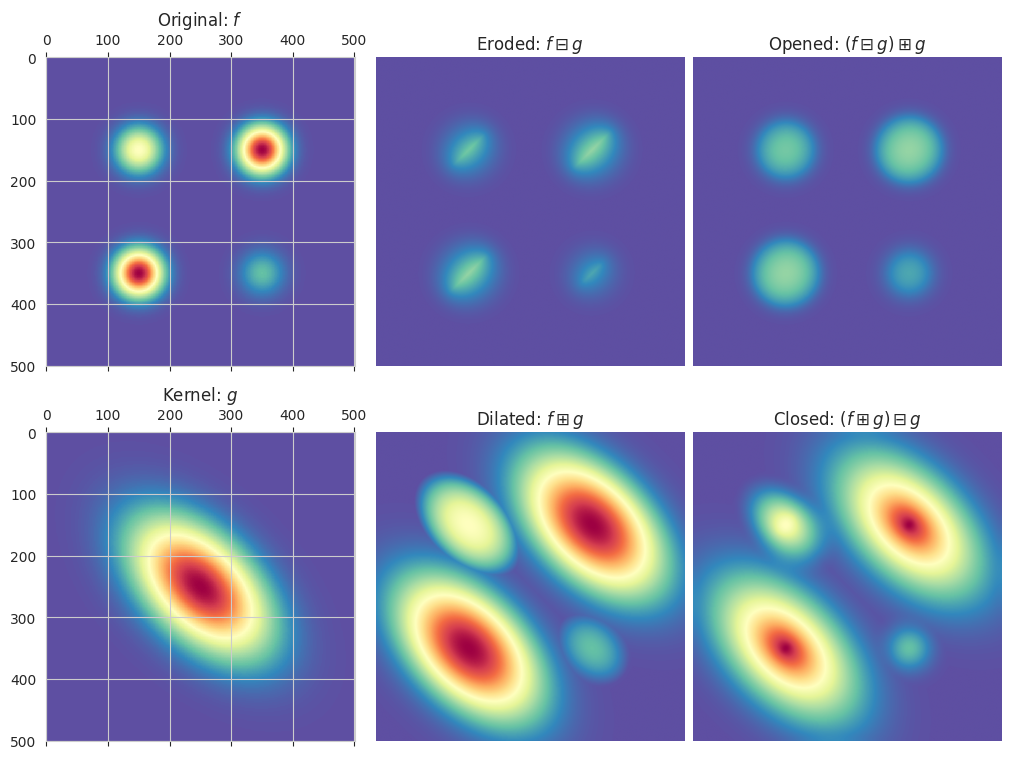
\includegraphics[width=\textwidth]{figures/morphological_2d.png}
  \caption{Illustration of the effects of dilation, erosion and their combination in two dimensions.}
  \label{fig:dil-illust}
\end{figure}
\comment{\ldots\ldots}


\chapter{Conclusion}


\bibliographystyle{ieeetr}
\bibliography{references}


\end{document}
